\chapter{THE LEXIMIN METHOD} \label{ch:algorithm}% Must have a blank line after every section label

\epigraph{Young man, in mathematics you don't understand things. You just get used to them.}{John von Neumann}

\noindent In this chapter, I describe the leximin method for hierarchical community detection. It relates a common problem in traffic engineering to the problem of community detection and finds communities in a divisive, hierarchical way. By maximizing all-pairs concurrent flow on the graph in an iterative process, edges become saturated with flow. At each level, these edges separate the graph into two or more parts. Flat clusters can be extracted based on some objective function; we select the clustering which maximizes modularity.

I define \say{leximin} and explain its connection to this problem. Next, I explain how the method identifies sparsest cuts to form a community structure. After defining the method, I illustrate the differences from the related MCF cut algorithm~\cite{mann2008extensions}. Finally, I give the computational complexity of the method as essentially $O(N^{11})$ in terms of the number of nodes $N$ and provide remarks to guide a practical implementation.



\section{Introduction}

The leximin method works to find cuts in the graph that separate it into well-connected subgraphs. The intuition of the method is a progressive filling process on a network of pipes~\cite{le2005rate}. 

\begin{method}{Progressive Filling~\cite{le2005rate}}

Begin with all rates equal to zero. Grow all rates at the same pace (or at a pace proportional to demand, when demand is not unity). Continue until one or more edges is saturated. These are the bottlenecks, or critical edges. The rates for demand pairs that use these links are now fixed: They do not increase anymore. Rates between other demand pairs continues to increase until a new bottleneck is found, and so on until the entire graph is saturated---all demand pairs have found a bottleneck. The process terminates because all edge capacities are finite and the graph is finite. The resulting allocation is max-min fair and unique~\cite{le2005rate}.
\end{method}

Matula first introduced the leximin method for community detection in 1985~\cite{matula1985divisive}. It rests on a hierarchical version of the maximum concurrent flow problem (MCFP) that was independently rediscovered nearly twenty years later by Nace and Doan in 2003~\cite{nace2003some}. In 2004, Allalouf and Shavitt made explicit the MCFP with non-unit demand which Matula identified in 1985 and Nace and Doan say is \say{easily generalized} from their model~\cite{allalouf2004maximum}. Much work has also built on Matula's MCFP, examining the simpler case that flow follows a fixed path or set of paths~\cite{pioro2003efficient, nace2003some, nace2006tutorial}.

The MCFP finds a fair allocation of flow between all pairs---that is, an allocation that is maximin maximal. When maximizing throughput between all pairs, a set of \emph{critical edges} will become fully saturated, corresponding to the idea of \emph{breakdown} in traffic theory: \say{the onset of congested traffic in an initial free traffic flow}~\cite{kerner2009traffic}. Because of these bottlenecks, there is residual capacity that can be utilized. The hierarchical MCFP (sometimes \say{lexicographically maximum concurrent flow problem}) utilizes that residual capacity to produce a max-min fair allocation---a leximin maximal satisfaction of demand.

The remainder of this chapter is structured as follows. In \autoref{sec:leximin_meaning}, we define \emph{leximin} as it pertains to flow networks. In \autoref{sec:sparsest cut}, we define sparsest cuts and show how they create a canonical hierarchical decomposition. In \autoref{sec:leximin algorithm}, we discuss the hierarchical maximum concurrent flow problem and how it is used to determine sparsest cuts and grids. \autoref{sec:differences} outlines the differences between the leximin method and the related MCF cut algorithm. Finally, in \autoref{sec:complexity and size}, we opine on the complexity, implementation, and practical limits of the algorithm.






\section{Leximin fairness} \label{sec:leximin_meaning}

The leximin method is so named because it identifies a lexicographic maximin (i.e.\ leximin) satisfaction of demand. A \emph{maximin} process is one that \emph{max}imizes the \emph{min}imum utility. For our purposes, utility and throughput are synonymous. A maximin flow allocation is one that has the highest minimum throughput. This is what the MCFP identifies. \emph{Lexicographic ordering} is a generalization of familiar alphabetic ordering: words are ordered by their first position, then their second, and so on. Lexicographic maximin extends the idea of maximin to multiple levels: we maximize the minimum utility, then for those who are not yet constrained, we maximize \emph{their} minimum utility, and so on. Economists have adopted the shorthand \say{leximin} because it is more economical in its number of syllables.

The leximin satisfaction of demand has a desirable property in traffic networks because it enforces \say{max-min fairness}. Bertsekas et al.~\cite{bertsekas1992data} discuss the idea of max-min fairness: that no pair's allocation can increase without reducing allocation to a pair with equal or lesser allocation. More casually, no-one can be made better off without taking from someone as well off or worse off. This is the same idea as leximin, and it is often an objective in bandwidth allocation for computer networks. Solving the hierarchical MCFP is a polynomial-time method for identifying such an allocation.







\section{The Sparsest Cut} \label{sec:sparsest cut}

On an unweighted graph (one with unit capacity on each edge), the sparsest cut is the minimal set of edges, with respect to the potential edges that could exist between the subgraphs it separates. In the case that an edge set~$\hat{E}$ cuts a graph into two parts~$A$ and~$\overline{A}$, the cut density is:

$$\frac{|\hat{E}|}{|A| \cdot |\overline{A}|}$$

The sparsest cut is the edge set~$\hat{E}$ that minimizes this value. Sometimes multiple cuts exist at a single level of throughput. Beyond the two-part case, the reader is referred to Mann~\cite{mann2008extensions, mann2008sparsest}. The edges that are not in $\hat{E}$ are non-critical. As there exists residual capacity on these edges after saturating the sparsest cut, the level of throughput can be raised on these edges. The pipes can keep being filled.



\subsection{The Sparsest Cut Hierarchy}

Beginning from the level of flow that saturated our sparsest cut, we keep filling the pipes, raising throughput. All the water already in the pipes is still there, eating up capacity. We approach a next-level bottleneck, and a next, until the entire network is partitioned into single nodes. Importantly, solving the hierarchical MCFP yields a unique dendrogram. The throughput continues to increase for each subproblem. Since the set of critical edges is canonical at every level, the dendrogram is canonical. The complication is in the case of ties, which cause \emph{degenerate cuts}: cuts at the same throughput value.

While a sparsest cut at a given throughput level~$z_i$ is not always unique, it is unique as long as there is no \emph{tie}, which is discussed in \autoref{ch:robustness}. When a tie occurs, the set of sparsest cuts is unique, and they will each be identified at the same throughput level~$z_i$. This guarantees a unique dendrogram, even in the face of ties.


In the following section, we discuss how the leximin method uses the hierarchical MCFP to find sparsest cuts and yield the dendrogram.






\section{The Leximin Method for Community Detection} \label{sec:leximin algorithm}

This algorithm identifies communities by identifying sparsest cuts in the graph. To find hierarchical structure, this can be repeated until the graph is decomposed into singletons. A flat structure can be extracted that maximizes some measure of community quality, such as stability of clusters~\cite{mcinnes2017hdbscan} or modularity~\cite{newman2006modularity}. Some of these measures allow early stopping, rather than generating the entire top-down structure. Identifying sparsest cuts is NP-hard~\cite{shahrokhi1990maximum, matula1990sparsest}, but the maximum concurrent flow problem (MCFP) can identify a class of sparsest cuts (\say{bottlenecks}) in polynomial time~\cite{matula1990sparsest}. 




\subsection{The MCFP and hierarchical MCFP}

The MCFP is a multicommodity flow problem with demand between all pairs of nodes in the network~\cite{matula1985concurrent}. The MCFP maximizes \emph{concurrent} flow: flow is supplied between all pairs in proportion to the demand between them. With unit demand, this means that flow between all pairs must be equal. The ratio of supplied flow to demand is called \emph{throughput} or \emph{satisfaction ratio}, and it must be the same between all pairs. The MCFP maximizes this throughput under the constraints of capacity on the edges.

A problem instance is represented by the tuple $\left< G, c, d \right>$ where $G = (V, E)$ is a graph, $c$ is a function $c\colon \{i, j\}  \rightarrow c_e \  \forall \{i, j\} \in E$ which provides the capacity of each edge, and $d$ is a function $d\colon \{i, j\}  \rightarrow d_{ij} \  \forall \{i, j\} \in D$ which defines the demand between all pairs. ($D \subseteq V \times V$~is the set of node pairs with demand between them.) The standard formulation assumes unit capacity on each edge and unit demand between all pairs.

There exist multiple possible LP representations of the MCFP. While more compact, efficient methods have emerged, the edge--path formulation is the conceptually simplest:
\begin{align}
    \max z(G, c, d)  & && \text{throughput} \nonumber\\
    \mathrm{s.t.} \sum_{p \in P_{ij}} f_p &= zd_{ij} \forall \{i, j\} \in D && \text{fairness constraint} \nonumber\\
    \sum_{\{p \in P:\{i,j\} \in E_p\}} f_p &\leq c_{ij} \forall \{i, j\} \in E && \text{capacity constraint} \nonumber\\
    f_p &\geq 0,  p \in P && \text{non-negativity of flow} \label{eq:mcfp}
\end{align}
We seek to maximize the concurrent throughput~$z$. Our first constraint enforces proportional maximization: the proportion of demand satisfied is the same for all pairs. The throughput~$z$ is  the sum of flows~$f_p$ for every path~$p$ in the set of paths~$P_{i, j}$ between nodes~$i$ and~$j$ (i.e. the total satisfied demand between~$i$ and~$j$).

\subsection{Formulation of the Leximin Method by Linear Programming}

In the hierarchical form, we maximize not just concurrent flow, but lexicographic concurrent flow. Residual capacity is not wasted. Instead, we use it to raise throughput for demand pairs that have not been constrained. We do this by solving a new LP for each throughput level, depending on the previous LPs: 

\begin{align}
    \max z_n(G, c, d)  & && \text{throughput} \nonumber\\
    \mathrm{s.t.} \sum_{p \in P_{ij}} f_p &= z d_{ij} \forall \{i, j\} \in D_n && \text{fairness constraint} \nonumber\\
    \mathrm{s.t.} \sum_{p \in P_{ij}} f_p &= z_l d_{ij} \forall \{i, j\} \in D_l, l = 1,\ldots,D_{n-1} && \text{lower levels constraint} \nonumber\\
%    \sum_{\{p \in P:\{i,j\} \in E_p\}} f_p &\leq c_{ij} \forall \{i, j\} \in E \setminus \mathit{crit}_n && \text{free capacity constraint} \nonumber\\
    \sum_{\{p \in P:\{i,j\} \in E_p\}} f_p &\leq c_{ij} \forall \{i, j\} \in E && \text{capacity constraint} \nonumber\\
    f_p &\geq 0,  p \in P && \text{non-negativity of flow} \label{eq:mcfp}
\end{align}

%\todo{Please check the formula before I send it to the committee.} 
Here, $z_l$ is a constant: the throughput of the $l$th subproblem, which was identified previously. $D_n$ identifies the subset of demand pairs that has not yet been saturated in subproblem $n$, and $D_l$ is the set of edges saturated in subproblem $l$. Some capacity has been utilized to achieve the previous level of throughput. Discounting that from the network's capacity \say{leaves the water in the pipes}, so we find a next solution building from there. We also no longer seek to further maximize demand between pairs that have already been constrained by a bottleneck. Because there is a bottleneck separating those pairs, they could not be maximized anyway.


\subsection{Determining the Sparsest Cut from the Hierarchical MCFP}

There is a unique set of critical edges saturated to capacity by every optimal assignment of flows, and removing these critical edges partitions the graph into two or more components~\cite{matula1985concurrent}. The remaining edges are non-critical, and their residual capacity can be used to improve throughput for the remainder of the graph. This creates a new set of critical edges and a new division.

Sometimes, the entire edge set of a subgraph bounded by cuts is saturated. This is a phenomenon called \emph{gridlock}, which is particular to maximizing concurrent flow. The subgraph is sufficiently homogeneous that there is no need to further dissect it and identify further community structure. The gridlock phenomenon is explored in \autoref{ch:random}.

\subsection{Main Steps of the Leximin Method}

The following steps are the iterative procedure to identify hierarchical community structure by identifying a leximin allocation of concurrent flow.

\begin{algorithm}
	\caption{Leximin clustering method}
	\label{alg:hmcfp-cc}
		\KwData{A graph $G = (V, E)$, edge capacities $c$, demand pairs $d$}
		\KwResult{A clustering $\mathcal{C}(G)$}
		$n \longleftarrow 1$\;
		\While{$\exists d \in D$ not saturated} {
		    \textbf{Solve the hierarchical MCFP subproblem} $P_n$\;
		    Extract critical edges~$\hat{E}_n$: those with nonzero shadow prices\;
		    Reduce available capacity on edges by $z$\;
		    $\forall d \in D_n$: $\lambda_d \longleftarrow z$ \;
		    $i \longleftarrow n + 1$\;
		}
		The final assignment of flows is max-min fair, and the satisfied demand is leximin maximal. The critical edges and their corresponding throughputs $z_i$ define a hierarchical structure of cuts.
		\vspace{0.25cm}
\end{algorithm}

The final consideration in constructing the dendrogram is the height at which each community should be merged. This height is called the \emph{cophenetic distance}~\cite{sokal1962comparison}. In this method, arbitrarily broken ties are reconciled by using throughput~$z$ as the cophenetic distance, rather than simply the number of divisions that have occurred to this point. This means that the ties (explored in \autoref{ch:robustness}) are reconciled as a multiway split at the same height, rather than remaining arbitrarily broken. 





\section{Differences from the MCF Cut Algorithm} \label{sec:differences}

\begin{figure}
\centering
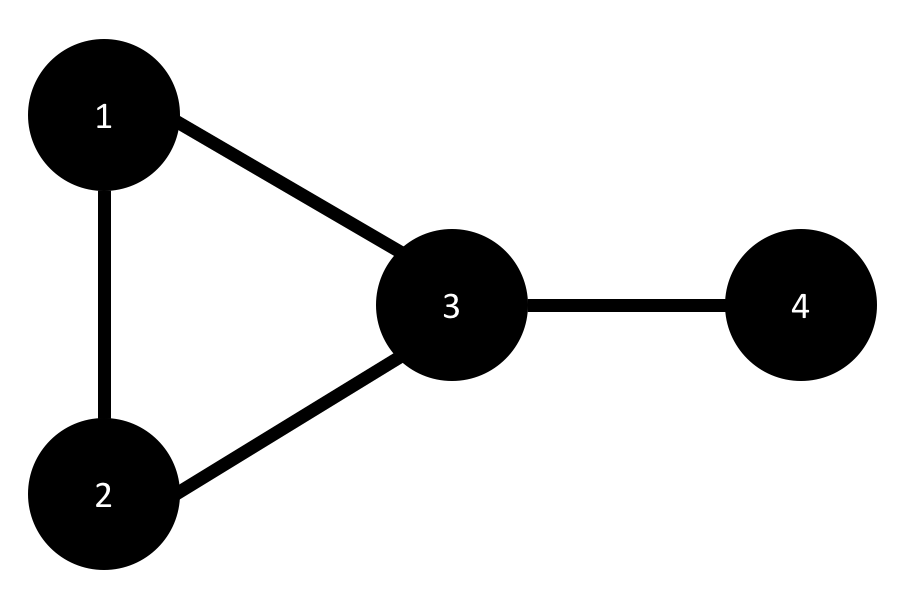
\includegraphics[width=0.6\textwidth]{fig/Paw3}
\caption{The paw graph}
\label{fig:paw3}
\end{figure}

\begin{figure}
\centering
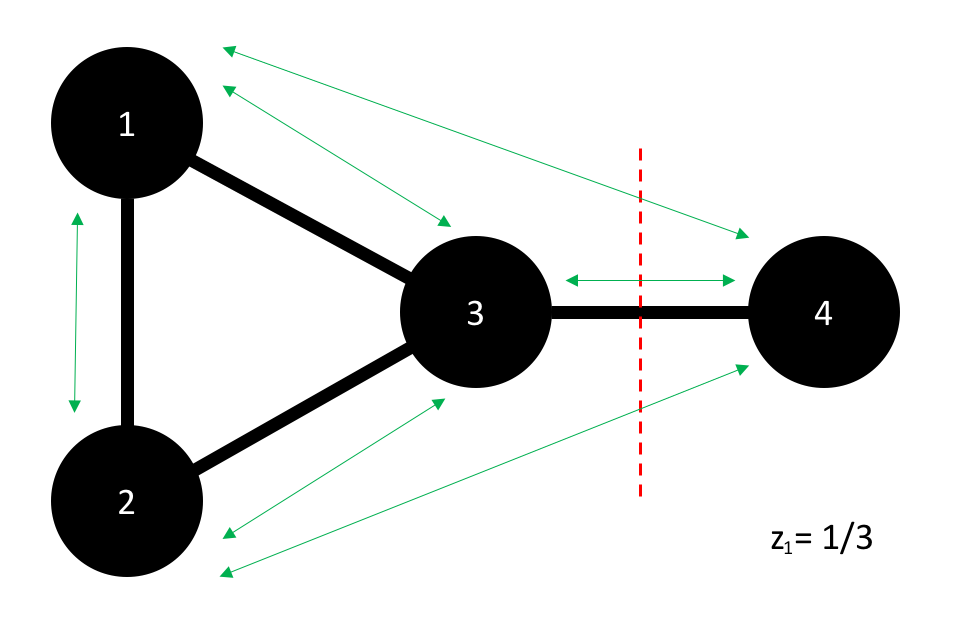
\includegraphics[width=0.6\textwidth]{fig/level1}
\caption{The first cut of the paw graph by the leximin algorithm. Green lines indicate paths of flow to fairly maximize minimum throughput. The red line indicates the cut.}
\label{fig:level1}
\end{figure}

\begin{figure}
\centering
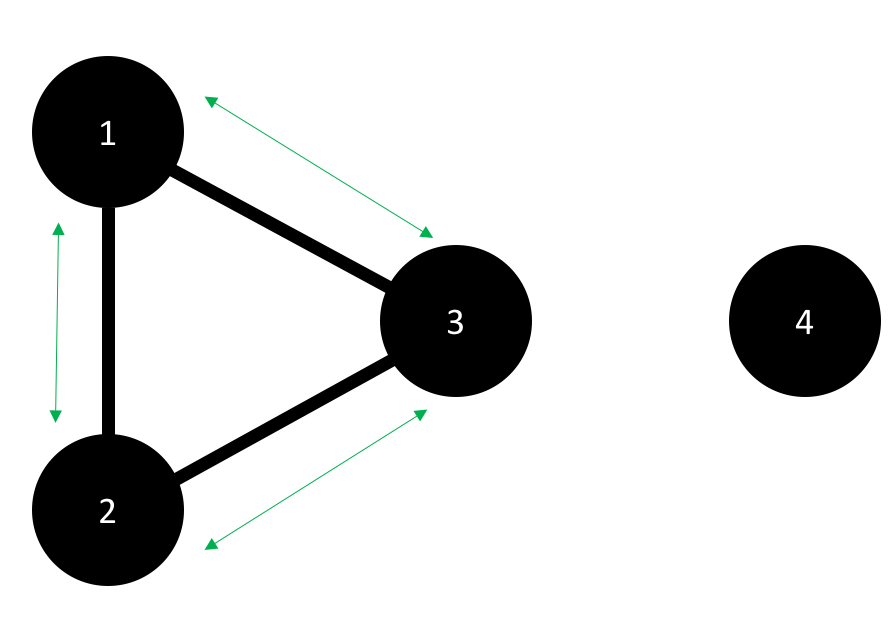
\includegraphics[width=0.6\textwidth]{fig/MCF_level2}
\caption{The subproblems for the MCF cut algorithm after its first cut: $K_3$ and a singleton}
\label{fig:MCF_level2}
\end{figure}

\begin{figure}
\centering
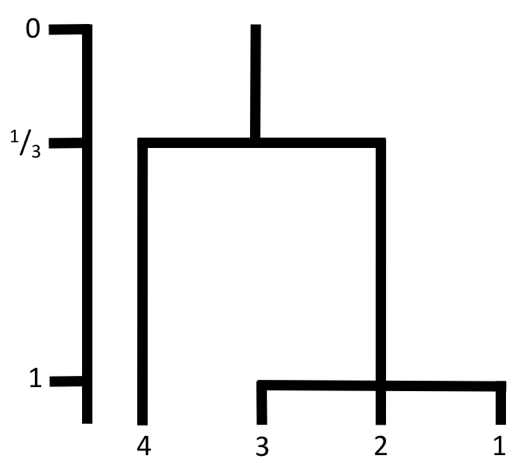
\includegraphics[width=0.4\textwidth]{fig/dendrogram_4_tie}
\caption{The dendrogram produced by the MCF cut algorithm on the paw graph}
\label{fig:MCF_dendrogram}
\end{figure}

\begin{figure}
\centering
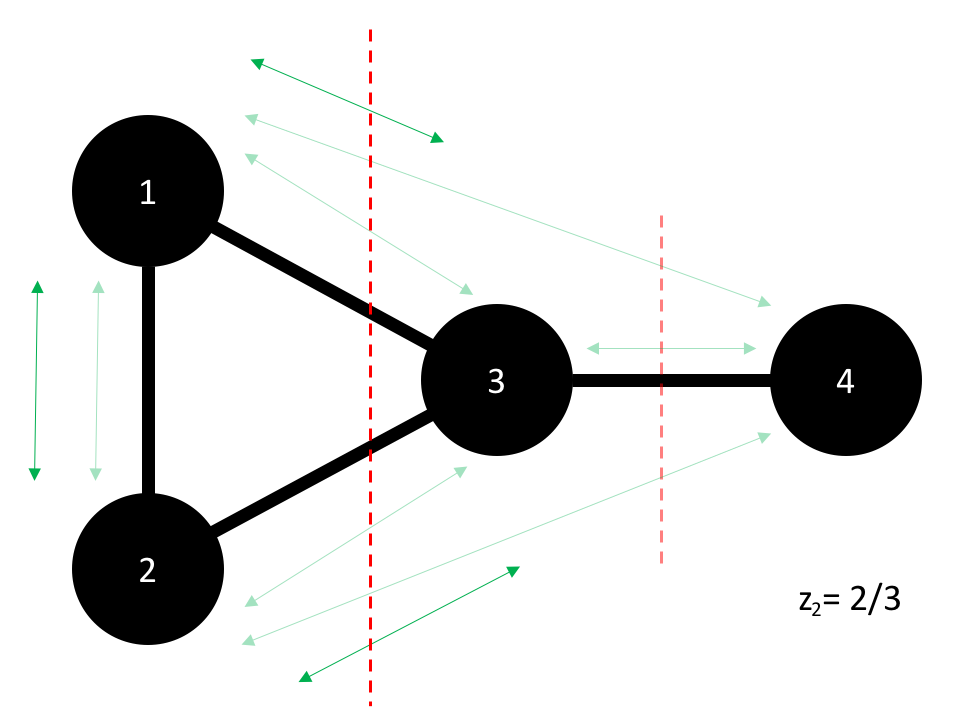
\includegraphics[width=0.6\textwidth]{fig/level2}
\caption{The second cut of the paw graph by the leximin algorithm. Green lines indicate paths of flow to fairly maximize minimum throughput. Red lines indicate cuts. Lighter colors represent fixed flow and previous cuts.}
\label{fig:level2}
\end{figure}

\begin{figure}
\centering
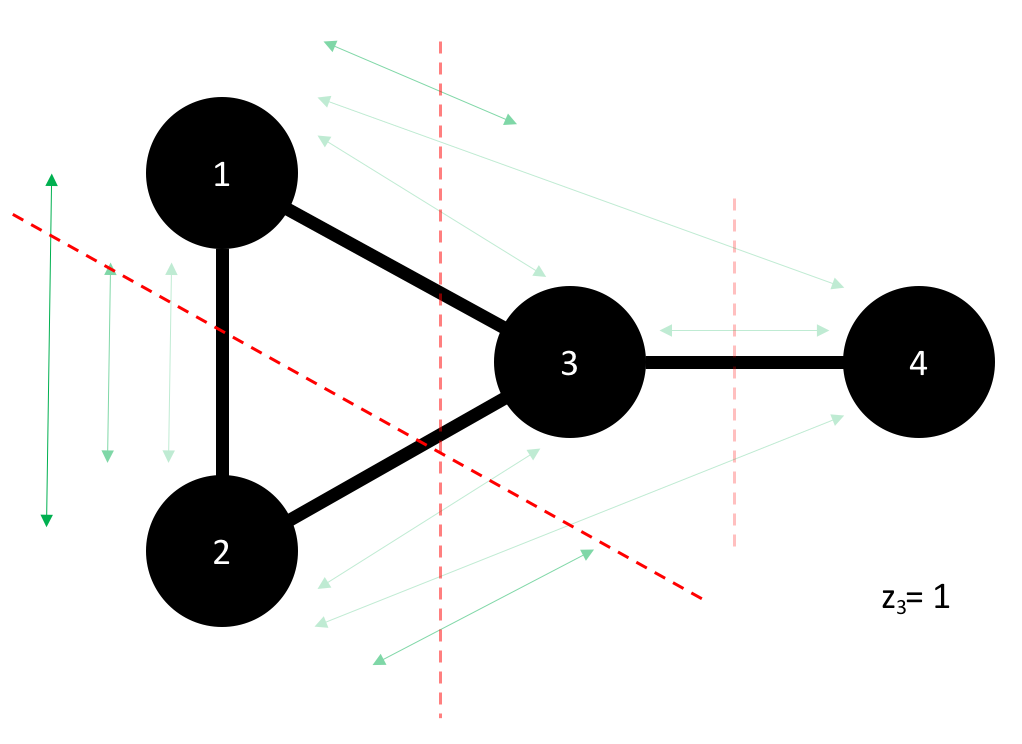
\includegraphics[width=0.6\textwidth]{fig/level3}
\caption{The third and final cut of the paw graph by the leximin method. The decision to cut $\{2, 3\}$ again instead of $\{1, 3\}$ is arbitrary.}
\label{fig:level3}
\end{figure}

\begin{figure}
\centering
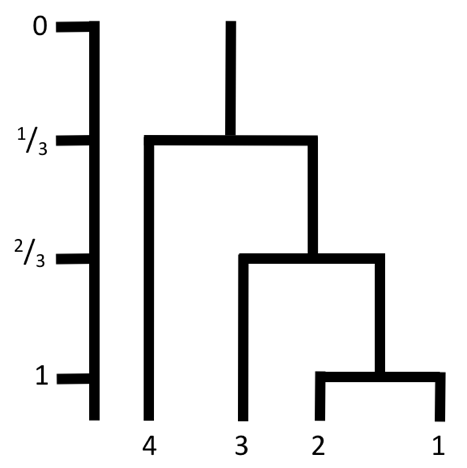
\includegraphics[width=0.4\textwidth]{fig/dendrogram_4_cascade}
\caption{The dendrogram produced by the leximin method on the paw graph}
\label{fig:leximin_dendrogram}
\end{figure}

The MCF cut algorithm is a similar technique to the leximin method which takes a divide-and-conquer approach~\cite{mann2008extensions}. It solves the MCFP on the network, then splits the network into components to process separately. This amounts to progressive filling up to the first bottleneck, then blocking the saturated pipes, draining the sections on each side, and starting anew on each side of the bottleneck. The components separated by the cut are re-solved independently of one another. This makes each subproblem smaller, but yields a different sequence of cuts and a different dendrogram.

The difference in behavior of the leximin and MCF Cut methods is best shown on a simple example. The paw graph is a graph formed by adding a fourth node to the complete graph $K_3$ and joining it to one of the existing vertices by an edge, as shown in \autoref{fig:paw3}.

The operation of the two algorithms begins identically; they differ in their treatment of subsequent steps. First, they progressively fill the network until an edge is saturated. Because this is the first iteration, there are no prior capacity usages in the leximin's hierarchical MCFP. This makes it equivalent to the MCFP solved in the MCF cut algorithm. \autoref{fig:level1} shows that the edge $\{3, 4\}$ (the \say{tail} of the paw graph) is saturated first, when there is $1/3$~unit of flow between all pairs. This edge is identified as critical. This is where the behavior deviates.

The MCF cut algorithm separates this graph into two subproblems: a triangle ($K_3$) and a singleton, as shown in \autoref{fig:MCF_level2}. When processing the triangle, we start from an initial state of no flow. Although the edge $\{1, 2\}$ had the least flow on it at the end of the first step, it is on equal footing with the other two edges of the triangle. The dendrogram for this method is then shown in \autoref{fig:MCF_dendrogram}.



In contrast to the MCF cut method, the leximin method does not remove flow already present in the network due to previous iterations. The starting point for the second iteration is shown in \autoref{fig:level2} as the lighter-colored lines. The flow required to saturate a new set of critical edges is shown in darker green. Here, there is an unambiguous next cut. The final edge is cut in \autoref{fig:level3}, which gives the final dendrogram: \autoref{fig:leximin_dendrogram}.

Because there is no clear definition of a community---and much less, a hierarchical communty---it is unclear which of these results is preferable. The leximin method has a clearer real-world significance, though: it partitions the graph based on the load applied to the graph. Further, the leximin method has desirable theoretical properties discussed in \autoref{ch:robustness}.


\section{Complexity and Size Considerations} \label{sec:complexity and size}

%The leximin algorithm is dramatically slower than competing algorithms, which can process networks with tens and hundreds of millions of nodes. The bulk of the mathematical effort  is solving the hierarchical MCFP. Proposals to increase this step's efficiency have been proposed. Dong et al.\ present the \say{triples} formulation of the MCFP, which drastically reduces the number of variables over the edge--path formulation, while also reducing the number of constraints~\cite{dong2015compact}.  Nevertheless, a dense network of 160 nodes can take an hour to process on current hardware. 

Solving a linear program is a polynomial-time technique, when inputs are algebraic numbers~\cite{adler1992polynomial}. The fastest known LP method has complexity $$O\left(\frac{n^3}{\log n}L\right)$$ where $n$ is the number of variables in the standard form of the LP and $L$ is the information length of the LP, which grows with the product of the number of variables and constraints~\cite{anstreicher1999linear}. In the efficient \say{triples} formulation of the MCFP, there are $O(mN)$ variables and $O(N^2)$ constraints. 

Since real-world networks have sparse connectivity~\cite{chakrabarti2006graph}, we can restrict our focus to these. Even on sparse graphs, solving an LP will take essentially $O(N^{10})$ time relative to the number of nodes in the graph. Given that up to $(N-1)$ LPs will be solved (one for each level of the hierarchy~\cite{nace2003some}), this amounts to a complexity of near $O(N^{11})$. The next slowest options are Walktrap ($O(N^{3.2})$) and Girvan--Newman ($O(N^3)$ on sparse graphs). 

\subsection{Practical Considerations for Implementation}
The edge--path form of the MCFP involves an exponential number of variables, which is untenable. Fortunately, more efficient representations have emerged. An implementer should prefer the triples formulation of the MCFP~\cite{dong2015compact}, which is easily extended to the hierarchical case. This method has a polynomial number of variables and constraints, yielding a tractable linear program in the complexity class P\@. Work to expedite handling degenerate cuts has also been done~\cite{danna2012practical}. The details of such a method, as well as its implementation, are out of the scope of this work.

Additionally, the method should only be applied to graphs of up to a few hundred nodes. On a sparse graph of 240 nodes, the runtime is measured in hours.

%\begin{algorithm}
%	\caption{MCF cut algorithm~\cite{mann2008extensions}}
%	\label{alg:mcf_cut}
%		\KwData{A graph $G = (V, E)$, edge capacities $c$, demand pairs $d$}
%		\KwResult{A clustering $\mathcal{C}(G)$}
%		$queue \longleftarrow \{G\}$
%		\While{$queue \neq \emptyset$}{
%			$H \longleftarrow queue.dequeue()$\;
%			\textbf{Solve the MCFP on $H$}\;
%		    Extract critical edges~$\hat{E}_i$: those with nonzero shadow prices \;
%		    \Unless{Something}{
%			\ForEach{component $H_j$ in $H$ cut by $\hat{E}_i$}{
%				$queue.enqueue(H_j)$\;
%			}}
%		}
%		\vspace{0.25cm}
%\end{algorithm}
